% =====================================================================
%  CAPÍTULO 5 — IMPLEMENTAÇÃO
% =====================================================================

\chapter{IMPLEMENTAÇÃO}
\label{cap:implementacao}

Este capítulo detalha a implementação do \argus{}, descrevendo a organização do
código-fonte, os principais módulos do \textit{backend} em Go e do
\textit{frontend} em JavaScript, as funcionalidades do sistema e os requisitos
atendidos.

\section{Visão geral do código}
\label{sec:visao-geral-codigo}

O repositório do projeto é organizado em três grandes áreas:

\begin{itemize}
    \item \code{app.go} e \code{gamification.go}: camada de aplicação
        exposta ao \textit{frontend} pelos \textit{bindings} Wails;
    \item \code{internal/}: núcleo do sistema, subdividido em \code{domain}
        (entidades e interfaces), \code{usecase} (fachadas), \code{service}
        (\code{ble}, \code{sim}, \code{gpx}, \code{fit}, \code{strava},
        \code{ai}, \code{workout}, \code{intervals}) e \code{repository}
        (persistência SQLite);
    \item \code{frontend/src/}: interface de usuário em JavaScript, com os
        módulos de controle (\code{modules/}), estilos (\code{styles/}) e
        componentes (\code{components/}).
\end{itemize}

Essa separação reflete a \textit{Clean Architecture} descrita no
Capítulo~\ref{cap:arquitetura} e viabiliza o desenvolvimento colaborativo e a
manutenibilidade do sistema.

\section{\textit{Backend} em Go}
\label{sec:backend}

\subsection{Módulo de conectividade BLE}
\label{sec:implementacao-ble}

O módulo \code{internal/service/ble} abstrai a comunicação com os sensores por
meio da biblioteca TinyGo Bluetooth \cite{tinygo2024}. Ele implementa o
escaneamento de dispositivos, a validação dos serviços GATT e a assinatura de
notificações para frequência cardíaca (\texttt{0x180D}), potência
(\texttt{0x1818}) e controle de rolos via FTMS (\texttt{0x1826}) e FE-C. A
comunicação é realizada por \textit{goroutines} concorrentes, de modo que a
recepção de telemetria não bloqueia a interface.

O módulo também disponibiliza um \textit{virtual trainer}, que simula o
comportamento de um rolo inteligente sem hardware físico, e \textit{mocks} para
viabilizar o desenvolvimento e os testes automatizados. Uma lista de dispositivos
BLE escaneados é exposta ao usuário por meio da interface de seleção explícita de
dispositivos.

\subsection{Motor de simulação física}
\label{sec:implementacao-sim}

O motor físico (\code{internal/service/sim}) implementa a equação de Martin
(Equação~\ref{eq:martin}) resolvida numericamente pelo método da bisseção, como
descrito na Seção~\ref{sec:equacao-martin}. A partir da potência instantânea
do atleta e do gradiente da rota, o motor calcula a velocidade virtual, que é
convertida em resistência mecânica enviada ao rolo em modo de simulação de
inclinação ou em potência alvo no modo ERG. O mesmo motor, portado para
JavaScript, é utilizado no aplicativo Android sem a necessidade do
\textit{backend} Go.

\subsection{Motor de métricas e exportação \texttt{.FIT}}
\label{sec:implementacao-fit}

O módulo \code{internal/service/fit} processa o vetor de \textit{samples} de
telemetria de \SI{1}{\hertz} e calcula as métricas fisiológicas: Potência
Normalizada (NP), Fator de Intensidade (IF), \textit{Training Stress Score}
(TSS), \textit{Training Impulse} (TRIMP) pela fórmula de Banister, tempo em
zonas de frequência cardíaca, recordes de potência (curva MMP) e o desvio
cardiovascular (Pw:HR). A biblioteca \code{muktihari/fit} \cite{fitgo2024} é
utilizada para serializar os dados no formato binário padrão Garmin/ANT+
\cite{garmin2024}, gerando arquivos compatíveis com Strava, Garmin Connect e
TrainingPeaks.

\subsection{Integração com serviços externos}
\label{sec:implementacao-externos}

A integração com o Strava (\code{internal/service/strava}) implementa o fluxo
OAuth 2.0 com \textit{refresh token} automático, utilizando um servidor HTTP
local para o \textit{callback} de autenticação. O \textit{upload} de atividades
é assíncrono e resiliente: falhas de rede são registradas em uma fila de
sincronização (\code{SyncQueue}) persistida no SQLite, com novas tentativas
programadas. A integração com o Intervals.icu
(\code{internal/service/intervals}) segue o mesmo padrão, ampliando a
interoperabilidade de dados do sistema.

\subsection{Assistente de treino com IA local}
\label{sec:implementacao-ai}

O assistente de IA (\code{internal/service/ai}) comunica-se com uma instância
do Ollama \cite{ollama2024} executada no dispositivo do usuário. O sistema
permite selecionar o modelo (por padrão, \texttt{qwen2.5:3b}), mantém o
histórico de conversas por perfil (\code{AIConversation}) e enriquece o
\textit{prompt} do sistema com os dados do atleta (FTP, nível, metas e
histórico recente de treinos). A partir da conversa, o assistente gera planos
de treino estruturados que são serializados no formato ZWO
(\code{saveWorkoutZWO}) e podem ser carregados diretamente no simulador em modo
ERG com um único clique.

\section{\textit{Frontend}}
\label{sec:frontend}

\subsection{Arquitetura e barramento de eventos}
\label{sec:frontend-eventbus}

O \textit{frontend} é implementado em JavaScript puro com Vite. O
\code{TelemetryEventBus} (em \code{frontend/src/modules/TelemetryEventBus.js})
desacopla a recepção de telemetria da renderização: os dados chegam do
\textit{backend} via \textit{bindings} Wails (ou do serviço BLE nativo do
Capacitor no Android) e são distribuídos aos assinantes (HUD, gráficos e
mapa) sem provocar \textit{reflows} globais, garantindo renderização fluida
a 60~fps.

\subsection{Mapa 3D e HUD}
\label{sec:frontend-mapa}

A renderização geográfica é realizada pelo MapLibre GL JS \cite{maplibre2024}
com terreno topográfico (Terrain-RGB), projeção globo 3D e temas claro/escuro.
A rota percorrida é colorida dinamicamente conforme o gradiente (verde para
trechos planos e vermelho para subidas íngremes), com o ciclista interpolado a
60~fps. O HUD exibe potência, cadência, frequência cardíaca, velocidade,
distância, elevação, zonas de potência e a barra de XP, com variações
especializadas para o modo Estúdio e para os modos de evento.

\subsection{Módulos de funcionalidades}
\label{sec:frontend-modulos}

O \textit{frontend} organiza as funcionalidades em módulos dedicados,
incluindo \code{MapController} (mapa e rota), \code{WorkoutController}
(treinos estruturados), \code{ChallengeController} (desafios e eventos),
\code{SummaryController} (resumo pós-treino), \code{AIChatController}
(assistente de IA), \code{FullscreenHUDController} (HUD em tela cheia),
\code{CapacitorBluetoothService} (BLE no Android) e \code{UIManager}
(orquestração da interface).

\section{Funcionalidades do sistema}
\label{sec:funcionalidades}

\subsection{Perfis de usuário e persistência local}
\label{sec:func-perfis}

O sistema suporta múltiplos perfis de atletas no mesmo dispositivo, cada um com
dados, nível, XP, FTP, peso e histórico de atividades isolados. A persistência
é 100\% local e \textit{offline-first}, com bancos SQLite dedicados para
atividades, recordes de potência, gamificação e eventos.

\subsection{Simulação e conectividade}
\label{sec:func-simulacao}

O \argus{} conecta-se a rolos inteligentes (FTMS e FE-C), medidores de potência
e cintas de frequência cardíaca, além de oferecer o \textit{virtual trainer}.
A resistência do rolo é controlada dinamicamente conforme o gradiente da rota,
o peso do atleta e o modo selecionado (ERG ou simulação de inclinação). A
Figura~\ref{fig:screenshot-telemetry} ilustra a telemetria em tempo real durante
uma sessão.

\begin{figure}[htbp]
    \centering
    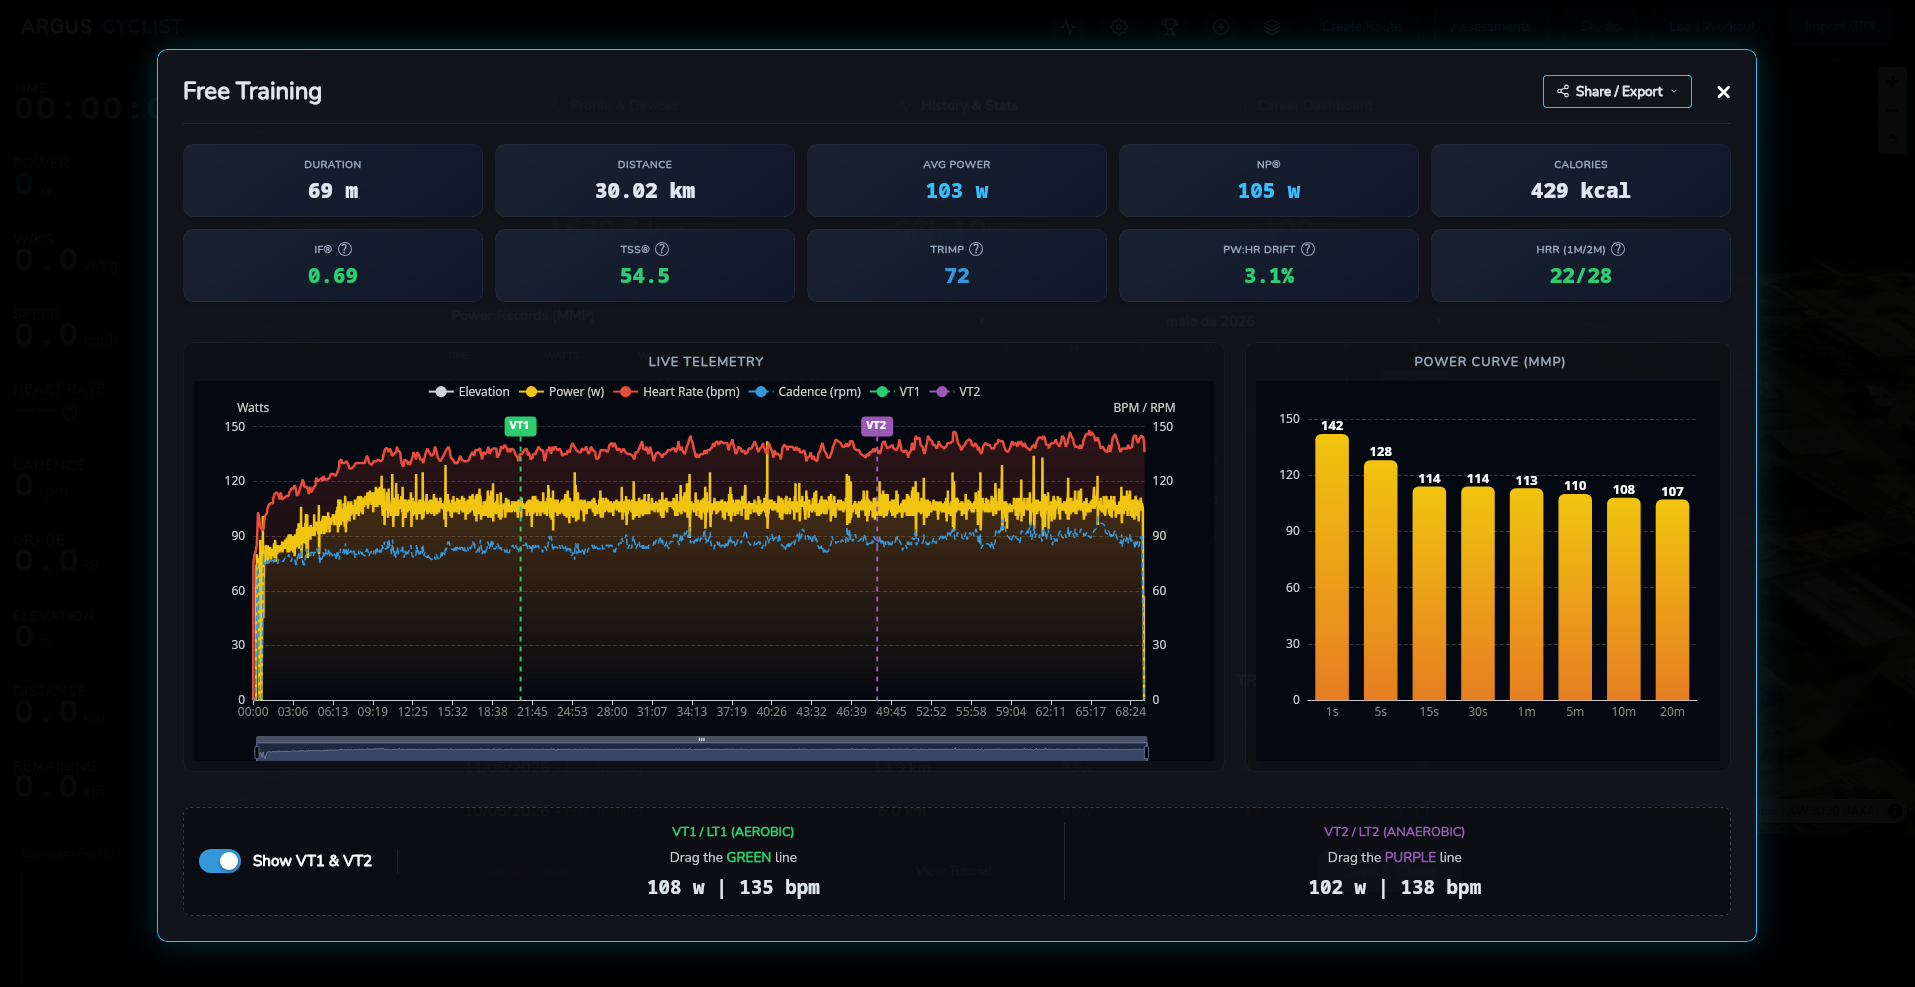
\includegraphics[width=0.85\textwidth]{figuras/screenshot-05-telemetry}
    \caption{Tela principal do simulador durante a sessão: telemetria em
    tempo real e mapa 3D}
    \label{fig:screenshot-telemetry}
    \small Fonte: autoria própria.
\end{figure}

\subsection{Treinos estruturados e avaliações de aptidão}
\label{sec:func-treinos}

Além do passeio livre, o sistema importa planos de treino ZWO e exibe os alvos
de potência em modo ERG, com ajuste de intensidade em tempo real. Avaliações
estruturadas de aptidão (\textit{Ramp Test} e teste de FTP) permitem estimar a
potência funcional limiar e calibrar as zonas de treino. A Figura~\ref{fig:screenshot-workout}
apresenta a execução de um treino estruturado.

\begin{figure}[htbp]
    \centering
    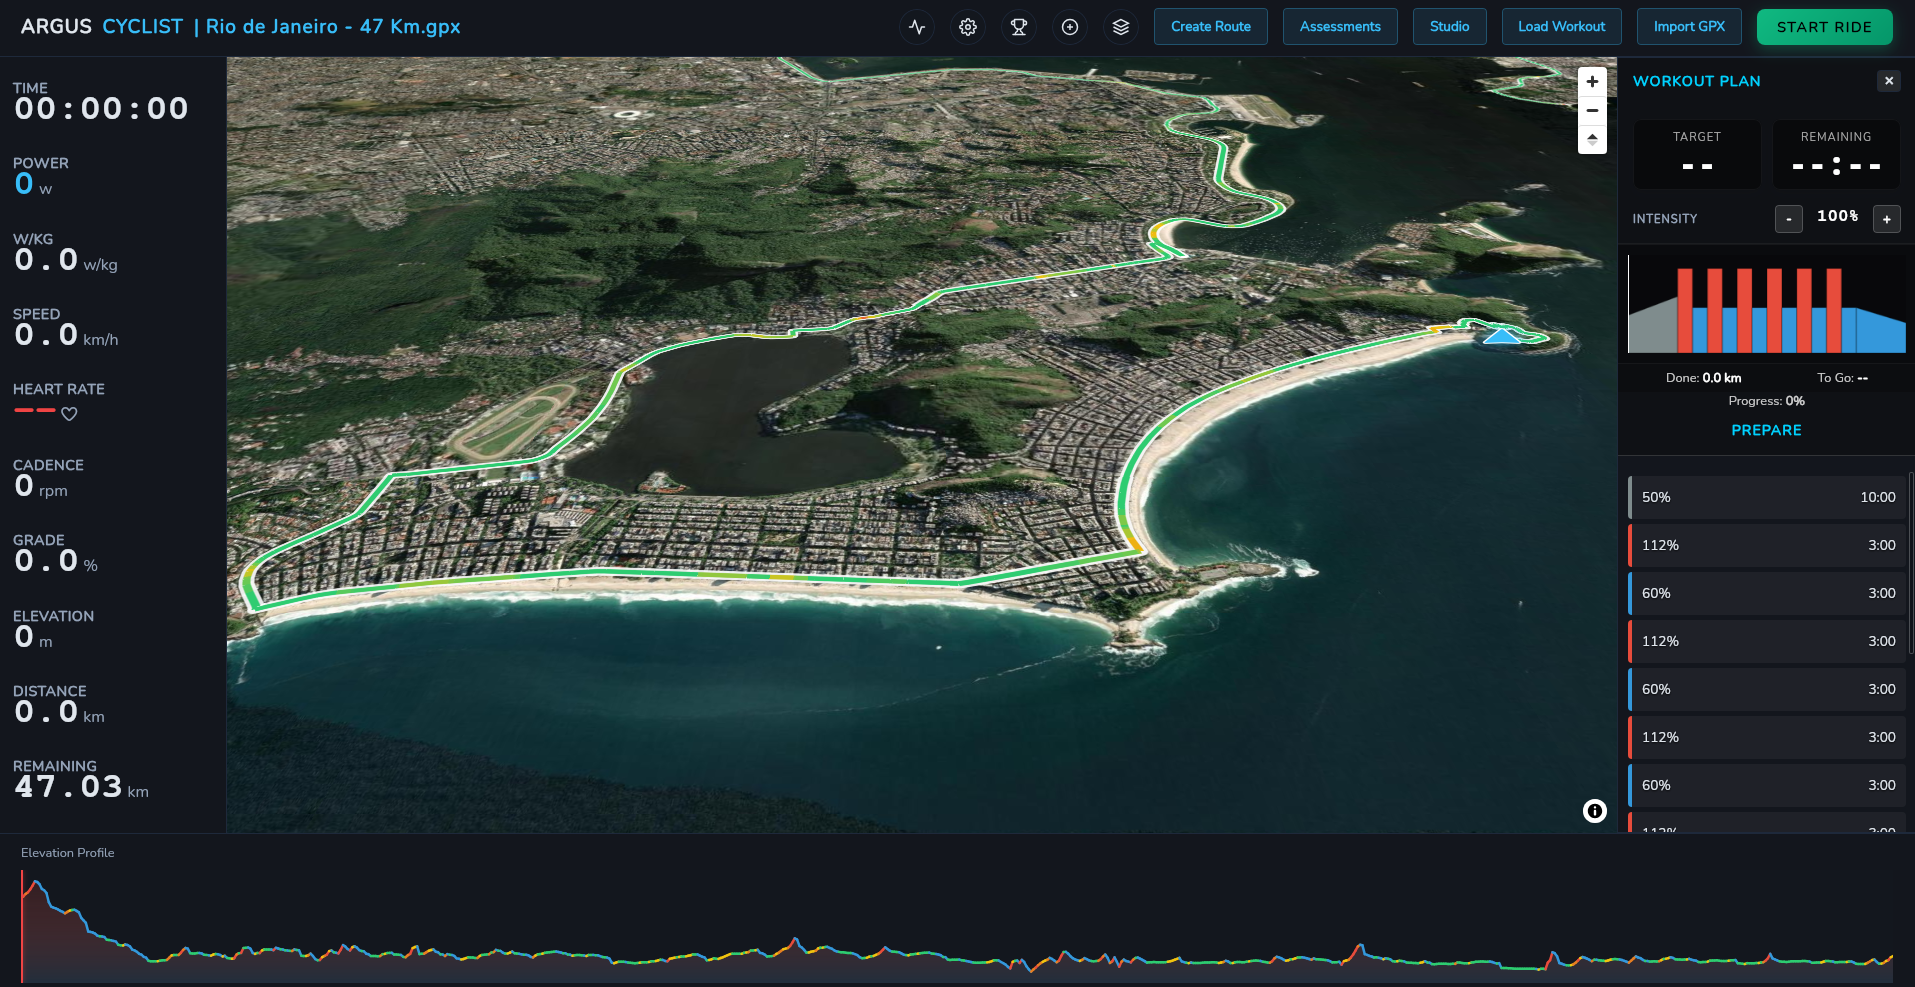
\includegraphics[width=0.85\textwidth]{figuras/screenshot-06-workout}
    \caption{Treino estruturado com alvo de potência em modo ERG}
    \label{fig:screenshot-workout}
    \small Fonte: autoria própria.
\end{figure}

\subsection{Modo Estúdio}
\label{sec:func-estudio}

O modo Estúdio (\textit{Studio Mode}) oferece um HUD dedicado à telemetria,
otimizado para aulas coletivas, com alvos de intervalo, zonas de potência e
cronômetros, sem o mapa 3D. A Figura~\ref{fig:screenshot-studio} ilustra esse
modo.

\begin{figure}[htbp]
    \centering
    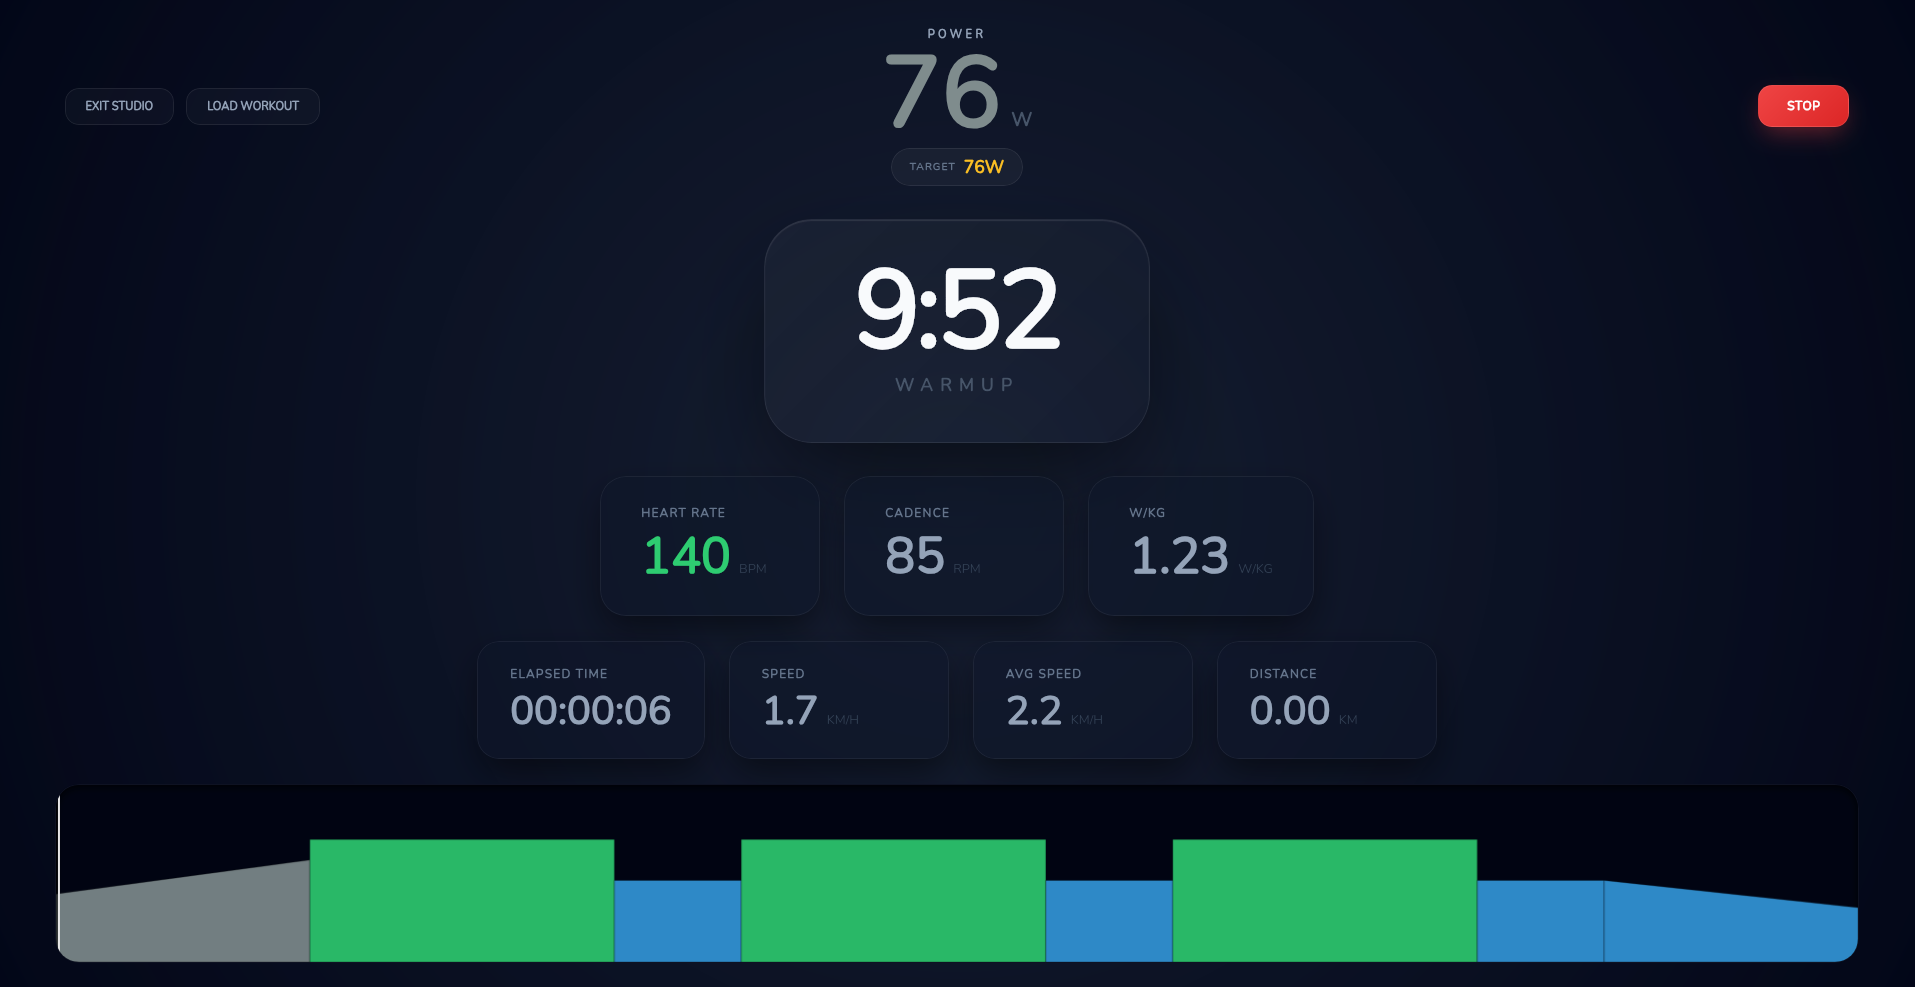
\includegraphics[width=0.85\textwidth]{figuras/screenshot-08-studio}
    \caption{Modo Estúdio: HUD de telemetria dedicado}
    \label{fig:screenshot-studio}
    \small Fonte: autoria própria.
\end{figure}

\subsection{Modo Evento}
\label{sec:func-evento}

O modo Evento (\textit{Event Mode}) permite a competição em desafios virtuais de
Sprint, KOM (\textit{King of the Mountain}) e Contrarrelógio (\textit{Time
Trial}), com regras de validação específicas e \textit{leaderboard} local
persistido em SQLite dedicado, incluindo filtros por gênero. A
Figura~\ref{fig:screenshot-event} apresenta a tela do modo evento.

\begin{figure}[htbp]
    \centering
    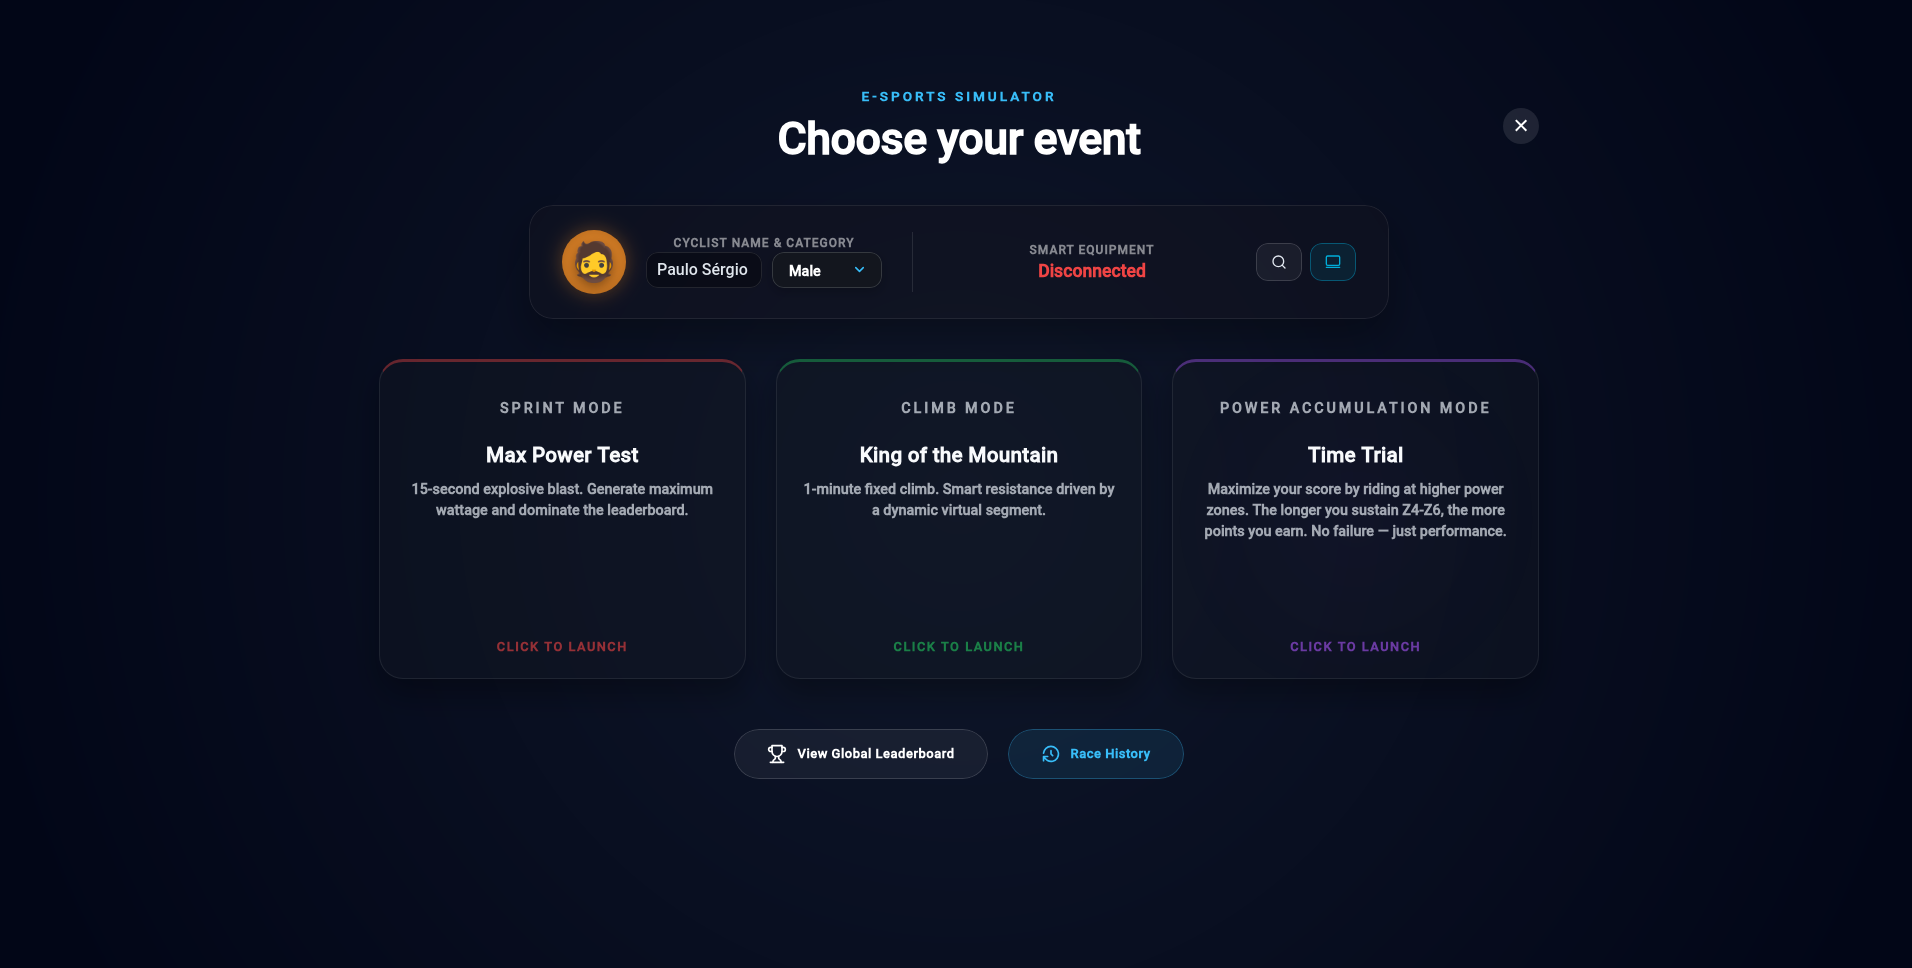
\includegraphics[width=0.85\textwidth]{figuras/screenshot-09-event}
    \caption{Modo Evento: desafio virtual com classificação local}
    \label{fig:screenshot-event}
    \small Fonte: autoria própria.
\end{figure}

\subsection{Gamificação}
\label{sec:func-gamificacao}

O sistema de gamificação (\code{gamification.go}) atribui XP passivamente
durante os treinos, com recompensas adicionais para subidas e longas
distâncias. Níveis, troféus, conquistas de consistência/recuperação/rotina e
metas personalizadas (\code{CustomGoal}) são persistidos por perfil e exibidos
na \textit{Trophy Room} (Figura~\ref{fig:screenshot-trophy}).

\begin{figure}[htbp]
    \centering
    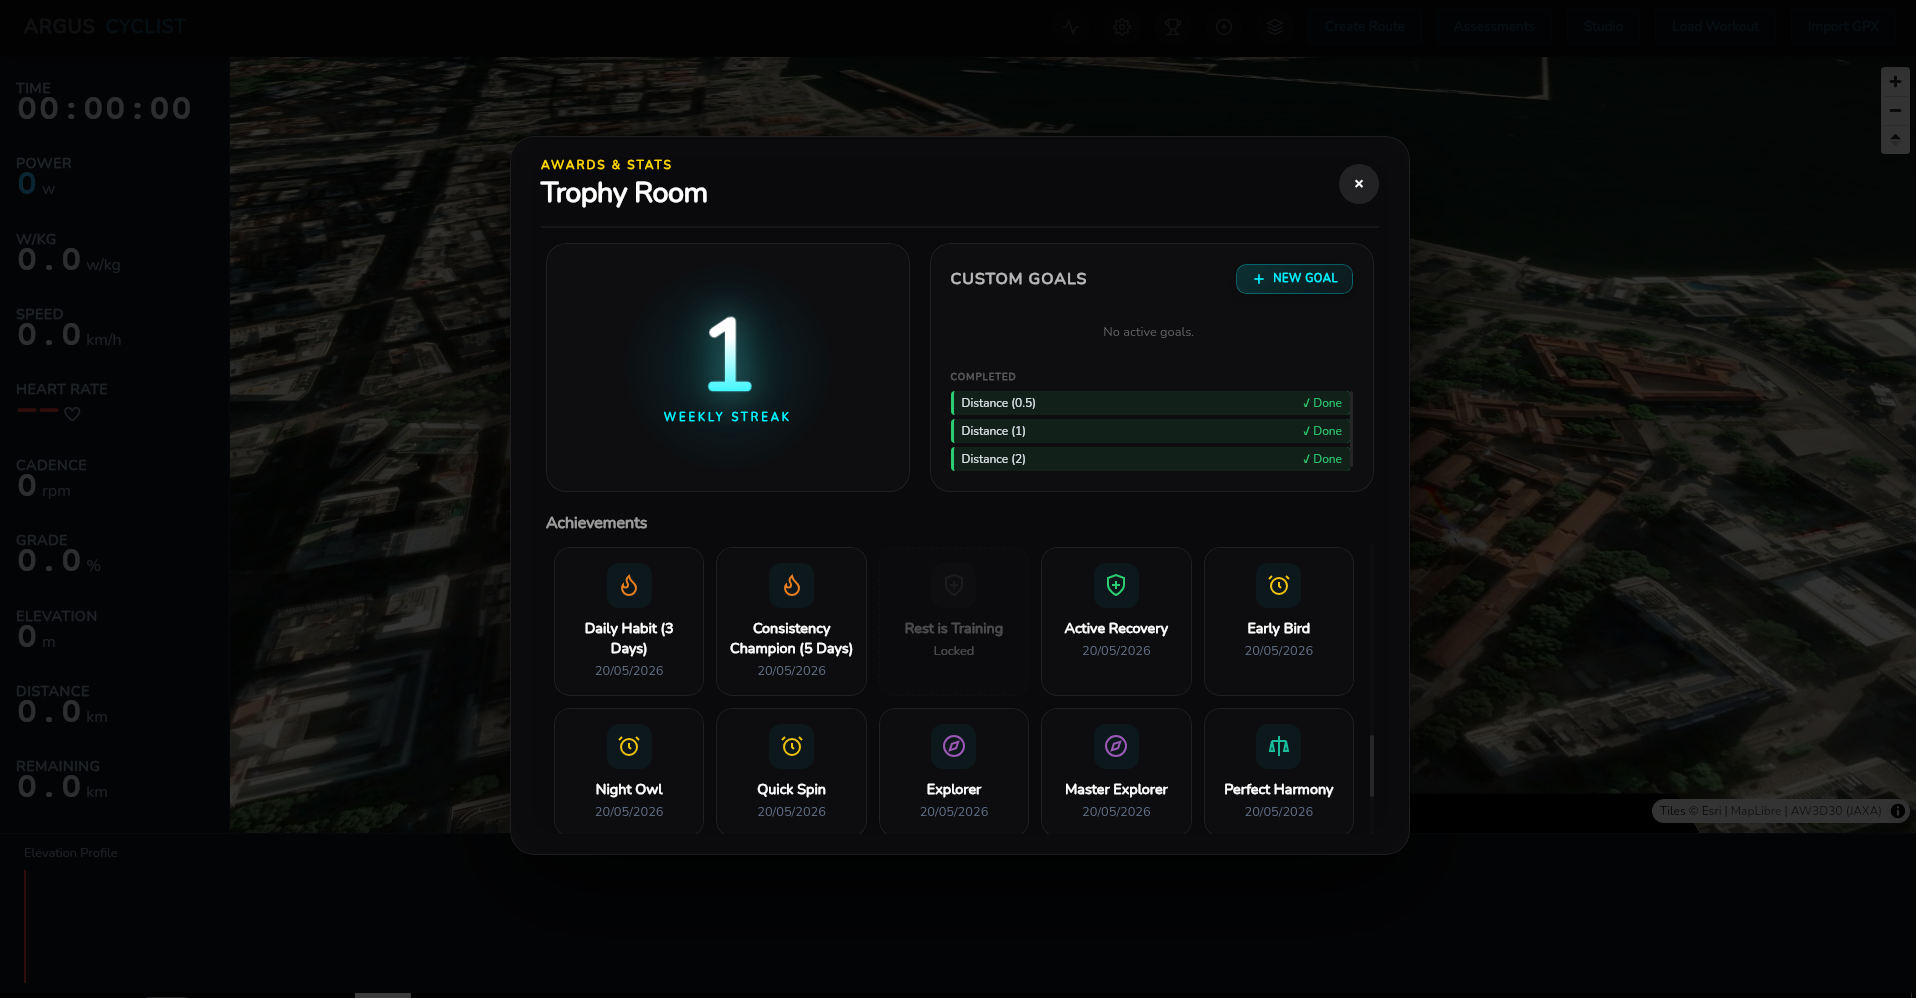
\includegraphics[width=0.85\textwidth]{figuras/screenshot-07-trophy}
    \caption{Trophy Room: troféus e conquistas do atleta}
    \label{fig:screenshot-trophy}
    \small Fonte: autoria própria.
\end{figure}

\subsection{Assistente de treino com IA}
\label{sec:func-ia}

O assistente de treino permite conversar em linguagem natural com um modelo de
linguagem local (Ollama), que considera o perfil do atleta e o histórico
recente para sugerir treinos e gerar planos ZWO carregáveis no simulador. As
conversas são persistidas por perfil e o modelo é selecionável pelo usuário.

\subsection{Rastreamento de desgaste de componentes}
\label{sec:func-componentes}

O módulo de componentes (\code{BikeComponent}) permite cadastrar peças da
bicicleta (corrente, cassete, coroas, etc.) com vida útil estimada em
quilômetros. Ao final de cada sessão, o desgaste é atualizado automaticamente
pela razão entre a distância acumulada e a vida útil, com indicadores visuais
codificados por cores (verde, amarelo e vermelho) e histórico de substituições
(\code{ComponentReplacement}) com auditoria temporal. A
Figura~\ref{fig:screenshot-desgaste} apresenta a tela de rastreamento de
componentes.

\begin{figure}[htbp]
    \centering
    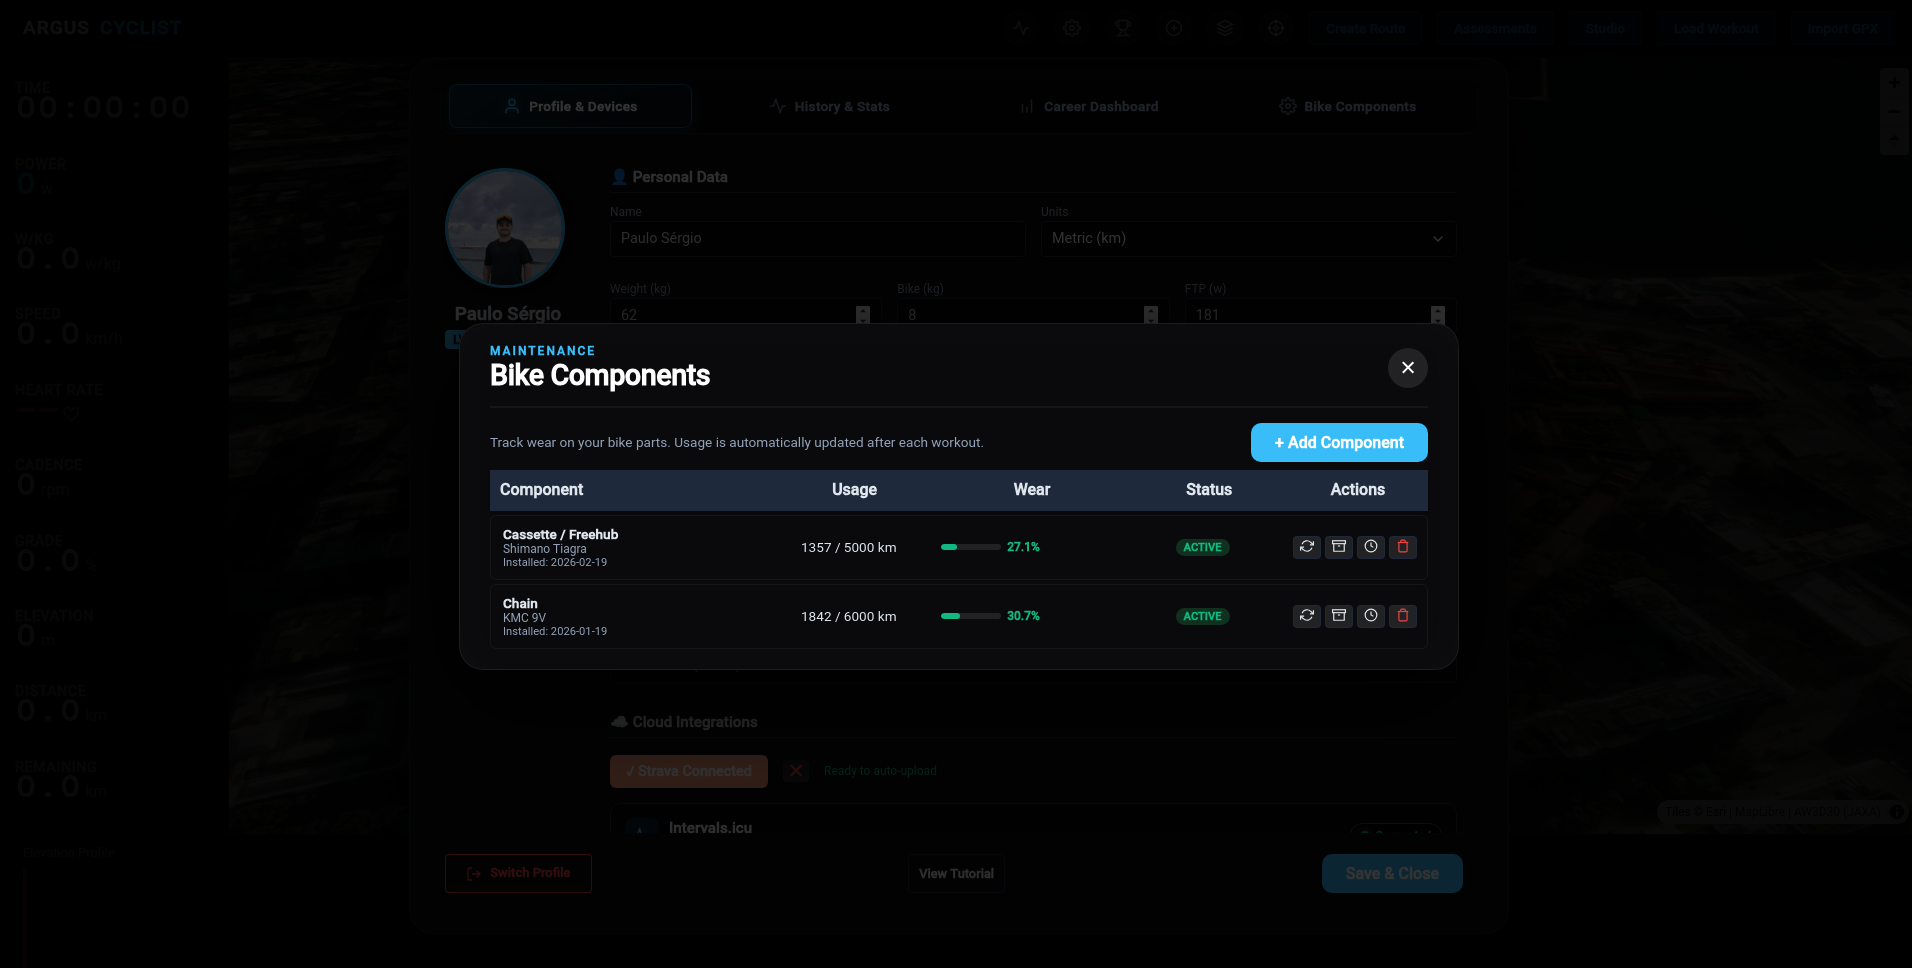
\includegraphics[width=0.85\textwidth]{figuras/screenshot-11-desgaste}
    \caption{Rastreamento de desgaste de componentes mecânicos}
    \label{fig:screenshot-desgaste}
    \small Fonte: autoria própria.
\end{figure}

\section{Requisitos funcionais e não funcionais}
\label{sec:requisitos}

A especificação de requisitos foi derivada da necessidade de estabilidade em
tempo real e de conformidade com os padrões de arquivos esportivos. As Tabelas
\ref{tab:rf} e \ref{tab:rnf} apresentam os requisitos funcionais e não
funcionais do sistema.

\begin{table}[h]
    \centering
    \caption{Requisitos funcionais do \argus{}}
    \label{tab:rf}
    \small
    \begin{tabular}{
        >{\raggedright\arraybackslash}p{4.2cm}
        >{\raggedright\arraybackslash}p{10.2cm}
    }
        \toprule
        \textbf{Identificador} & \textbf{Descrição} \\
        \midrule
        RF01 & Gestão de sensores BLE: escaneamento, pareamento e recepção de
        dados via perfis GATT de frequência cardíaca, potência e cadência. \\
        RF02 & Controle de equipamento (FTMS/FE-C): envio de comandos de
        resistência para rolos inteligentes em modo ERG ou simulação de
        inclinação. \\
        RF03 & Motor de simulação GPX: interpretação de rotas GPX e cálculo da
        velocidade virtual baseado no peso do atleta, potência e inclinação. \\
        RF04 & Registro de atividade (FIT SDK): geração de arquivos binários
        \texttt{.fit} com todos os \textit{samples} de telemetria da sessão. \\
        RF05 & Integração Strava: autenticação OAuth 2.0 e \textit{upload}
        automático de sessões finalizadas. \\
        RF06 & Persistência local: armazenamento de usuários, configurações,
        histórico de atividades e recordes em SQLite local. \\
        RF07 & Desafios e gamificação: desafios de segmentos (Sprints e KOM) e
        avaliações de capacidade (teste FTP) durante a simulação. \\
        RF08 & Assistente de IA local: geração de planos de treino ZWO
        personalizados via Ollama. \\
        RF09 & Controle de desgaste de componentes: cadastro e cálculo automático
        de desgaste de peças com histórico de substituições. \\
        RF10 & Integração Intervals.icu: \textit{upload} de atividades
        finalizadas. \\
        \bottomrule
    \end{tabular}
\end{table}

\begin{table}[h]
    \centering
    \caption{Requisitos não funcionais do \argus{}}
    \label{tab:rnf}
    \small
    \begin{tabular}{
        >{\raggedright\arraybackslash}p{4.2cm}
        >{\raggedright\arraybackslash}p{10.2cm}
    }
        \toprule
        \textbf{Identificador} & \textbf{Descrição} \\
        \midrule
        RNF01 & Latência de telemetria: o tempo entre a recepção do pacote BLE e
        a atualização na interface não deve exceder \SI{150}{\milli\second}. \\
        RNF02 & Portabilidade: a base de código deve ser compilável para Windows
        (Wails), Linux e Android (Capacitor) sem perda de funcionalidades. \\
        RNF03 & Estabilidade de conexão: rotinas de auto-reconexão para sensores
        que percam sinal durante a sessão. \\
        RNF04 & Eficiência de memória: o \textit{backend} em Go não deve exceder
        \SI{200}{\mega\byte} de \textit{footprint} durante a simulação ativa. \\
        RNF05 & Privacidade: processamento local de dados biométricos, com
        integrações externas apenas sob consentimento explícito do usuário. \\
        RNF06 & Licenciamento: distribuição sob licença GPLv3
        \cite{gpl2007}. \\
        \bottomrule
    \end{tabular}
\end{table}
